\item A sleeve \( A \) can slide freely along a smooth rod bent in the shape of a half-circle of radius \( R \) (Fig. 1.28). The system is set in rotation with a constant angular velocity \( \omega \) about a vertical axis \( OO' \). Find the angle \( \theta \) corresponding to the steady position of the sleeve.
    \begin{center}
        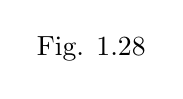
\begin{tikzpicture}
            \node at (0, 0) {Fig. 1.28};
        \end{tikzpicture}
    \end{center}